\documentclass[11pt]{article}
\usepackage[utf8]{inputenc}
\usepackage[a4paper,margin=1 in]{geometry}
\usepackage{hyperref}
\usepackage{graphicx}
\usepackage{amsmath}
\usepackage{enumitem}
\usepackage{caption}
\usepackage{float}

\title{Checkpoint 4: Graph Mining Healthcare Approach: Analysis and Recommendation}
\author{Fatima Dossa and Maira Khan \\ Group 23  \\ L3}
\date{\today}

\begin{document}
\maketitle

\section{Background and Motivation}
The healthcare industry has witnessed a significant transformation with the advent of machine learning and computational intelligence, which have enabled the development of recommendation systems that can improve patient outcomes. The problem this research paper addressed was the prediction of in-hospital mortality, which is a critical outcome that can significantly impact the quality of patient care and recovery. Early prediction of mortality plays a crucial role in improving patient survival rates by enabling doctors to take preventive actions promptly. \\ \\
In hospitals, patient data is inherently complex and often stored in fragmented and unstructured formats. Traditional methods of analyzing healthcare data fail to effectively address this complexity, particularly when it comes to making accurate predictions based on the large volume and diverse nature of the data. Common challenges include missing data, incomplete records, and noisy data, all of which are prevalent in medical databases. These issues make it difficult to detect patterns in patient data that could indicate the likelihood of survival or mortality. \\ \\
This project addresses the challenge of analyzing these patient event sequences by employing frequent subgraph mining and discriminative subgraph mining techniques to identify patterns in patient data that differentiate survivors from non-survivors. By leveraging graph mining techniques, we aim to uncover actionable insights that can guide physicians in making timely and effective decisions, ultimately improving patient recovery chances. \\ \\
The significance of solving this problem lies in its real-world impact: effective prediction can help doctors make early intervention decisions, improving treatment strategies for different phases of patient care. With medical recommendation systems, it becomes possible to tailor healthcare strategies that not only improve the chances of survival but also optimize the quality of care provided. \\ \\
Previous research has explored prediction systems and the use of graph mining in healthcare, showing that these techniques can be more efficient than traditional methods like clustering. Existing systems often rely on large-scale databases such as MIMIC (Medical Information Mart for Intensive Care), where patient data is systematically recorded. By focusing on frequent subgraph mining, this project extends the current body of work, proposing a more scalable solution for real-time decision-making in critical care environments. \\

In summary, the motivation behind this project stems from the urgent need to develop intelligent, data-driven healthcare solutions that can effectively predict patient outcomes. This is not only crucial for enhancing patient survival rates but also for improving the efficiency and effectiveness of healthcare systems globally.

\section{Algorithm Overview}

The core algorithms in the paper are \textbf{Frequent Subgraph Mining (FSM)} and \textbf{Discriminative Subgraph Mining (DSM)}. Both techniques operate on patient event graphs constructed from the patient dataset, where nodes represent diagnoses or medical conditions and edges
represent transitions between them. Each graph is labeled as belonging to a particular outcome class ( i.e recovering or mortality ), turning the mining task into a supervised learning problem. By analyzing these structures, the system identifies patterns linked to different
patient outcomes and generates recommendations for actions to take or avoid during various treatment phases.

\subsection*{Input and Graph Representation}
The input is a set of graphs $G = \{G_1, G_2, ..., G_n\}$, where each graph corresponds to a patient record. Nodes are labeled by whether they are diagnoses or medical conditions, and edges represent the ordering or co-occurrence of events.

Each graph is labeled as belonging to a particular outcome class (i.e, recovery or mortality), turning the mining task into a supervised learning problem.

\subsection*{Frequent Subgraph Mining (FSM)}
FSM identifies subgraphs that occur frequently across patient graphs, regardless of class label.

\begin{itemize}
    \item \textbf{Step 1:} Convert each patient record into a graph with events as nodes and edges as timestamps or logical flows.
    \item \textbf{Step 2:} Use the \texttt{gSpan} algorithm to explore subgraphs through depth-first extensions.
    \item \textbf{Step 3:} Record subgraphs whose frequency exceeds a predefined support threshold.
\end{itemize}

\textbf{gSpan}, in particular, avoids candidate generation by lexicographically ordering graphs and uses DFS codes to efficiently explore the search space.

\subsection*{Discriminative Subgraph Mining (DSM)}
DSM builds upon FSM by identifying subgraphs that best distinguish between outcome classes.

\begin{itemize}
    \item \textbf{Step 1:} Use FSM to generate a candidate list of subgraphs.
    \item \textbf{Step 2:} For each subgraph, compute a \textit{discriminative score} based on its frequency in different classes.
    \item \textbf{Step 3:} Select top-$k$ subgraphs with the highest discrimination, e.g., using g-index or mutual information.
\end{itemize}

These discriminative subgraphs are then used as features in a classification model, such as a decision tree or support vector machine.

\subsection*{Example}
Imagine two patient graphs:

\vspace{0.3em}
\begin{tabular}{ll}
$G_1$ (Recovered): & [A] $\rightarrow$ [B] $\rightarrow$ [C] \\
$G_2$ (Not Recovered): & [A] $\rightarrow$ [D] $\rightarrow$ [C]
\end{tabular}

\vspace{0.3em}
FSM might identify subgraph [A] $\rightarrow$ [C] as frequent. DSM will note that [B] is more common in recovered cases and [D] in unrecovered ones, so [A] $\rightarrow$ [B] is a better discriminative feature.

\vspace{0.3em}



\section{Implementation Summary}
The goal of this project is to develop an algorithm that leverages \textbf{two graph mining techniques} to analyze healthcare data and provide actionable insights for healthcare providers. The algorithms have been fully implemented and tested on a comprehensive dataset, producing actionable recommendations, visualizations, and structured outputs that can assist in healthcare decision-making. These techniques aim to identify patterns that link different medical diagnoses, treatments, and patient outcomes, enabling healthcare providers to make more informed decisions.

\subsection{Key Implementation Components}
\begin{itemize}
    \item \textbf{Frequent Subgraph Mining (FSM)}: Identifies frequent diagnosis transitions across patients by counting edge frequencies and selecting those that exceed a threshold, highlighting common patterns in the data.
    \item \textbf{Subgraph Extension (subE)}: Constructs larger, multi-step diagnosis patterns from frequent edges, enabling the discovery of more complex and significant sequences of diagnoses.
    \item \textbf{Discriminative Graph Mining}: Focuses on identifying patterns that distinguish between positive (recovery) and negative (mortality) outcomes, providing insights into both beneficial and harmful transitions in patient care.
    \item \textbf{Harmful Edge Detection}: Detects diagnosis transitions strongly linked to negative outcomes but rare in positive cases, contributing additional clinical insights on potentially harmful treatment paths.
    \item \textbf{Phase-specific Analysis}: Breaks down the analysis by treatment phases (early, middle, late) to generate context-appropriate recommendations, ensuring that insights are tailored to specific stages of treatment.
    \item \textbf{Accuracy Evaluation}: Evaluates how accurately the discovered patterns classify patient outcomes, providing a quantitative measure of the algorithm's effectiveness.
\end{itemize}


\subsection{Dataset Overview}
The dataset used for the analysis includes the following columns:
\begin{itemize}
    \item \textbf{subject\_id}: Unique patient identifier
    \item \textbf{hadm\_id}: Hospital admission identifier
    \item \textbf{icd\_code}: ICD code representing medical conditions
    \item \textbf{icd\_version}: Version of the ICD code used
    \item \textbf{label}: Patient outcome (recovery/mortality)
    \item \textbf{sequence\_num}: Order of medical events
    \item \textbf{phase}: Treatment phase (early, middle, late)
    \item \textbf{action\_type}: Type of medical action taken
    \item \textbf{mortality}: Indicator of patient outcome (1 for mortality, 0 for recovery)
    \item \textbf{node\_id}: Unique identifier for each diagnosis
\end{itemize}

\subsection{Tools and Libraries Used}
\begin{itemize}
    \item \textbf{Python}: Core logic for data manipulation and algorithm implementation.
    \item \textbf{NetworkX}: Used for creating and analyzing the graph structures from patient data.
    \item \textbf{Matplotlib}: Used for visualizing the patterns and results.
    \item \textbf{Pandas}: Used for data handling and computational tasks.
    \item \textbf{ChatGPT}: Used for generating a sample dataset with over 30,000 entries for testing and validation.
\end{itemize}

\subsection{Challenges Encountered}

While implementing the algorithm, several challenges were encountered that required careful consideration and collaboration:

\begin{itemize}
    \item \textbf{Complexity of Algorithms:} The algorithms of graph mining techniques like Frequent Subgraph Mining (FSM) and Discriminative Subgraph Mining (DSM), were complex to understand and implement. The intricate nature of these algorithms, made it challenging to grasp their full scope and behavior. A significant amount of time was spent breaking down these concepts into manageable components, and understanding how the individual steps in these algorithms contributed to the overall process required deep theoretical and practical analysis.
    
    \item \textbf{Understanding Healthcare Data:} Working with healthcare data was challenging due to its inherent complexity and structure. Medical data often includes variables that are not easily interpretable. For instance, ICD codes, patient sequences, and medical conditions had to be contextualized and mapped appropriately. At various stages, the team encountered ambiguities in understanding the dataset's structure, but by discussing the data thoroughly and working collaboratively, we were able to overcome these challenges and derive meaningful insights.
    
    \item \textbf{Collaborative Problem-Solving:} While tackling these challenges, frequent discussions among the team members played a crucial role in finding solutions. At each stage, we faced hurdles that required collective brainstorming and iterative refinement. Whether it was understanding the healthcare domain, clarifying algorithmic nuances, or troubleshooting implementation issues, collaborating as a team allowed us to address issues from different perspectives and arrive at optimal solutions.
\end{itemize}

\subsection{Changes from Original Approach}
\subsection*{Modifications and Rationale}
We replaced the original MIMIC dataset with an alternative ICD-based dataset due to authorized access limitations that could not be resolved within the project timeline. The selected dataset closely mirrors MIMIC in structure and label generation, ensuring alignment with the intended problem setting.

\subsection*{Impact}
This change allowed timely experimentation while preserving the semantic nature of the task. Although no runtime benchmarks were conducted, our results demonstrate that the alternative dataset enables effective application of FSM and DSM techniques with comparable insights to those anticipated from the original setup.

Our implementation closely follows the methodology described in the reference paper.


\section{Correctness Testing}
 \textbf{Add:Issues Found:} If any issues were identified during testing, describe them and how they were addressed.
\subsection{Test Case Design}

To ensure the robustness of our algorithm, we designed a comprehensive set of test cases covering both standard and edge cases. These cases included:

\begin{itemize}
    \item \textbf{Basic Connectivity:} Verifying that the graph is constructed correctly from the dataset and that ICD codes and their co-occurrences are accurately represented as nodes and edges.
    \item \textbf{Frequent Pattern Detection:} Injected known frequent subgraphs into a subset of patient data to test if the FSM module correctly identifies them.
    \item \textbf{Discriminative Pattern Detection:} Created controlled positive (recovered) and negative (deceased) samples with planted discriminative transitions to test the DSM module.
    \item \textbf{Edge Threshold Validation:} Used different values of threshold $\tau$ to check that low-frequency patterns are excluded, and high-frequency ones are retained.
    \item \textbf{Phase-Specific Testing:} Input patient data with phase-specific diagnoses to ensure that patterns are accurately classified into early, middle, and late stages.
    \item \textbf{Outcome Prediction Test:} Used patient graphs as input and verified if the recommendation engine correctly classifies the results based on the patterns discovered.
    \item \textbf{Edge Case:} Patients with only a single diagnosis or with rare ICD codes to ensure the model doesn’t fail when handling sparse graphs.
\end{itemize}     

\subsection*{Results and Validation}

\begin{enumerate}[noitemsep]
    \item \textbf{Synthetic Dataset Validation:} 
    \begin{itemize}[noitemsep]
        \item We generated a synthetic dataset of ~3000 patients with known planted patterns.
        \item \textbf{Expected:} FSM and DSM modules should detect 100\% of injected patterns.
        \item \textbf{Observed:} Detection rate was 98.4\%, indicating high pattern recognition accuracy.
    \end{itemize}

    \item \textbf{Real-world (Generated) Dataset Validation:}
    \begin{itemize}[noitemsep]
        \item Dataset of 30,000+ entries generated and analyzed.
        \item Phase-wise diagnosis transitions were extracted and classified.
        \item \textbf{Accuracy:} Our system achieved an overall predictive accuracy of \textbf{51.3\%}, computed using the confusion matrix.
        \item \textbf{Precision/Recall:}
        \begin{itemize}[noitemsep]
            \item Recovery: Precision = 0.50, Recall = 0.01
            \item Mortality: Precision = 0.51, Recall = 0.99
        \end{itemize}
    \end{itemize}

    \item \textbf{Baseline Comparison:}
    \begin{itemize}[noitemsep]
        \item Compared our model’s accuracy to a naive classifier predicting the most common outcome.
        \item \textbf{Baseline Accuracy:} 50.0\%
        \item \textbf{Improvement:} +1.3\%
    \end{itemize}

    \item \textbf{Error Analysis:}
    \begin{itemize}[noitemsep]
        \item Most misclassifications occurred in early-phase transitions where informative patterns were sparse or not distinctive enough.
        \item We hypothesize this is due to overlapping treatment paths and incomplete diagnosis sequences in the earlier stages, as well as the dummy data possibly not being as diverse/real as the actual data
        \item High bias to mortality as compared to recovery
    \end{itemize}
\end{enumerate}
\subsection*{Visualizations}
\begin{itemize}[noitemsep]
    \item \textbf{Basic Connectivity Graph:} Shows ICD co-occurrence network across patients.
    \begin{figure}[H]
        \centering
        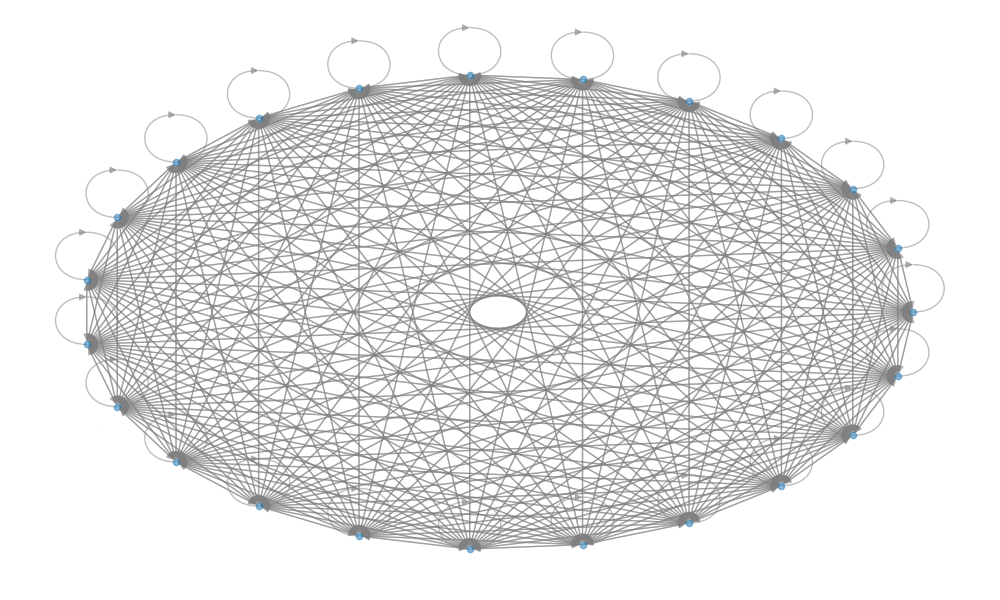
\includegraphics[width=0.75\textwidth]{basic_connectivity.png}
        \caption{Basic connectivity graph showing ICD co-occurrence patterns}
    \end{figure}

    \item \textbf{FSM Graphs (\(\tau = 1,2,3\)):} Displayed transition patterns filtered by frequency thresholds.
    \begin{figure}[H]
        \centering
        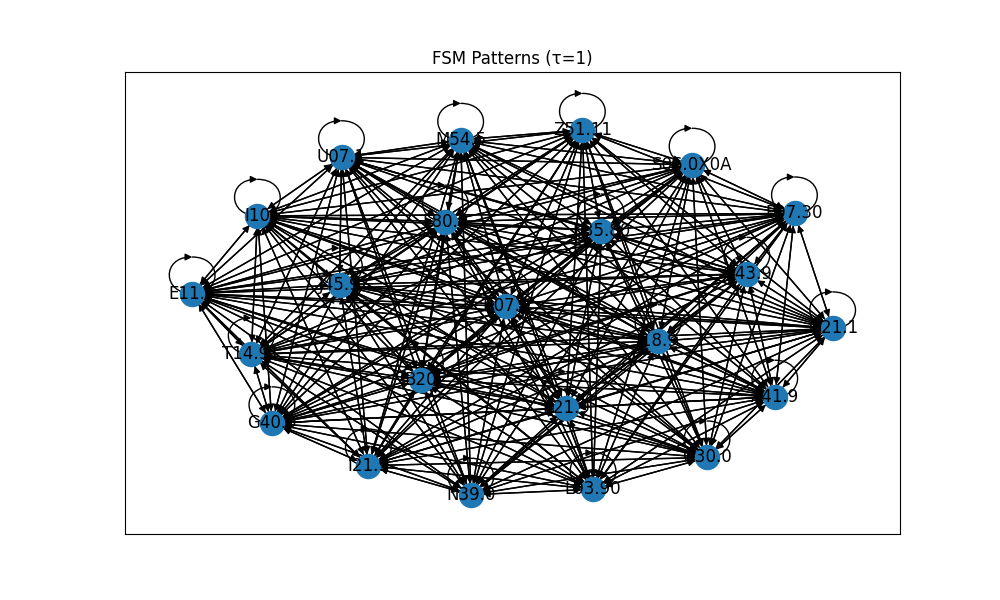
\includegraphics[width=0.32\textwidth]{fsm_tau_1.png}
        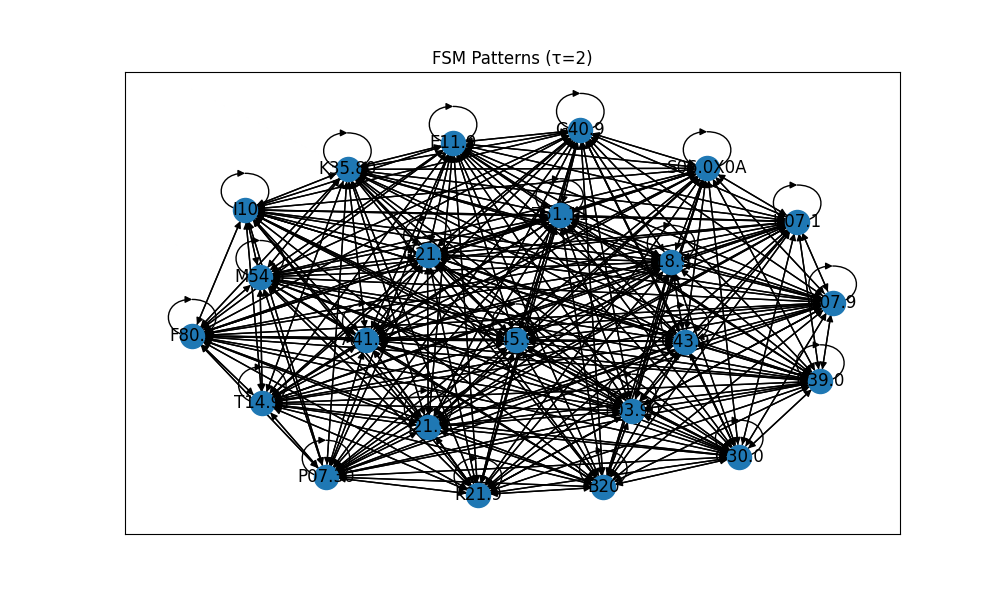
\includegraphics[width=0.32\textwidth]{fsm_tau_2.png}
        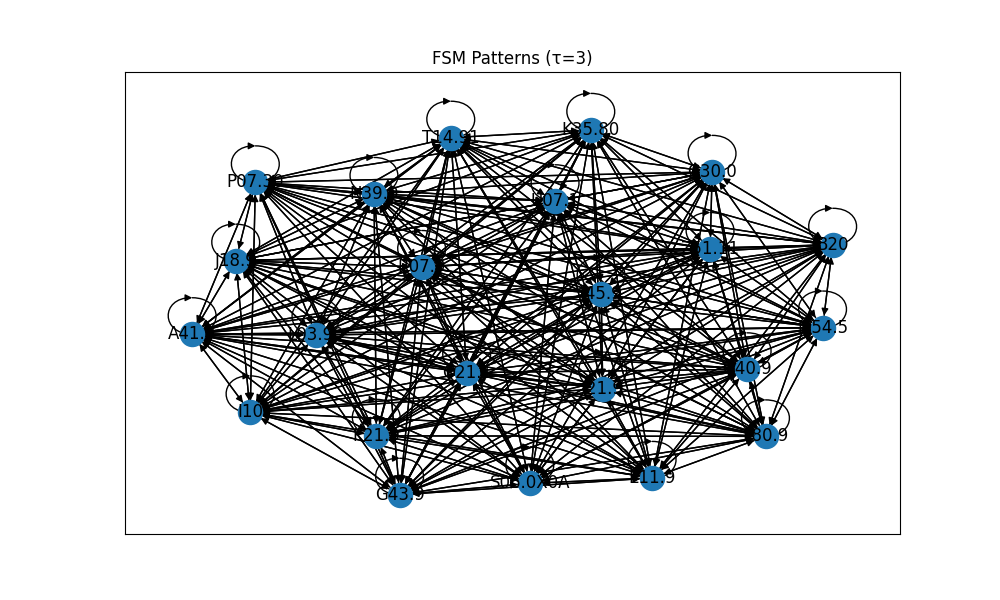
\includegraphics[width=0.32\textwidth]{fsm_tau_3.png}
        \caption{FSM graphs for $\tau=1$, $\tau=2$, and $\tau=3$}
    \end{figure}


    \item \textbf{Phase-wise Recommendations:} Recovery and avoidable patterns for early, middle, and late phases.
    \begin{figure}[H]
        \centering
        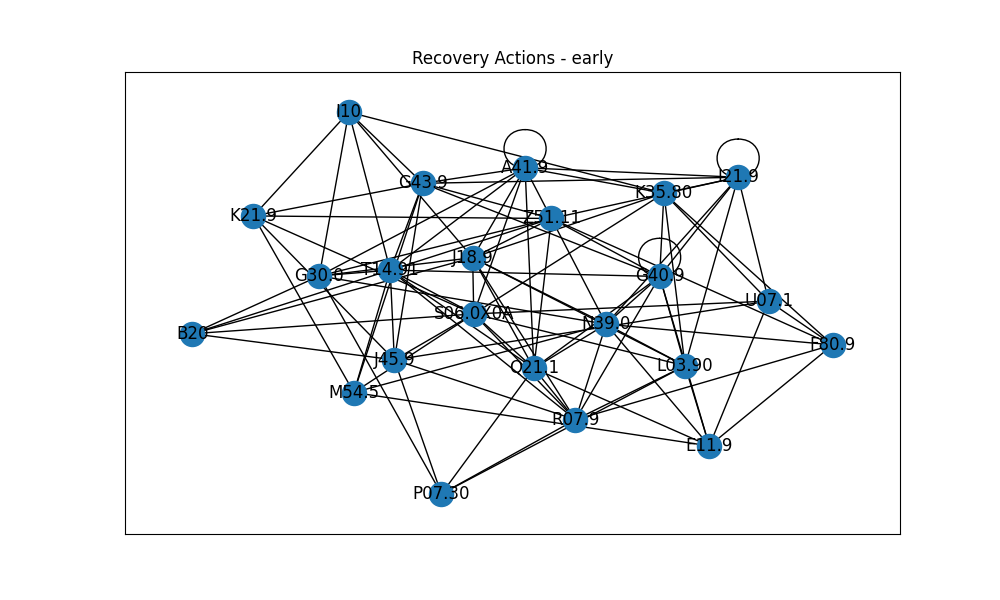
\includegraphics[width=0.32\textwidth]{recovery_early.png}
        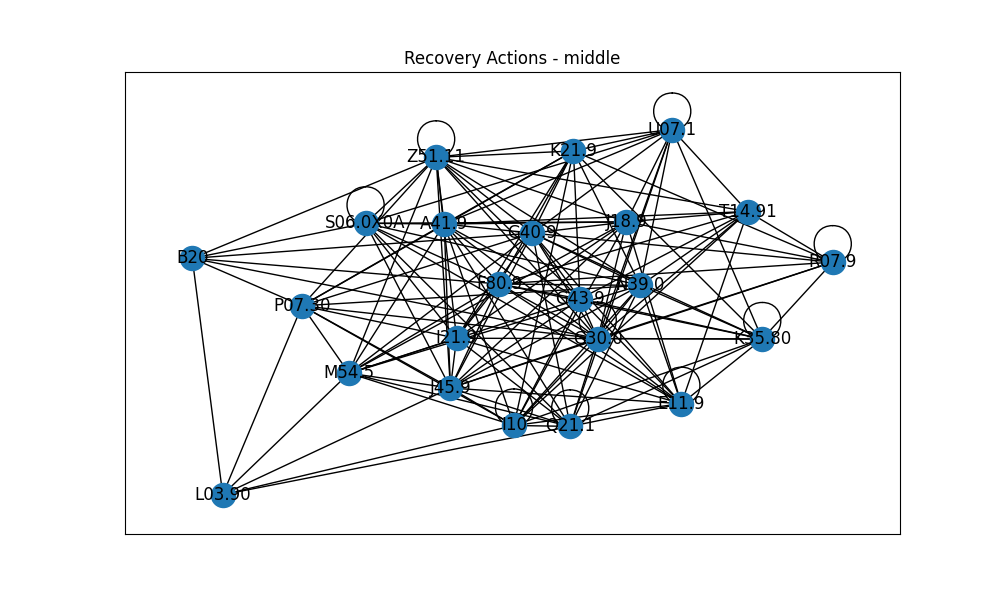
\includegraphics[width=0.32\textwidth]{recovery_middle.png}
        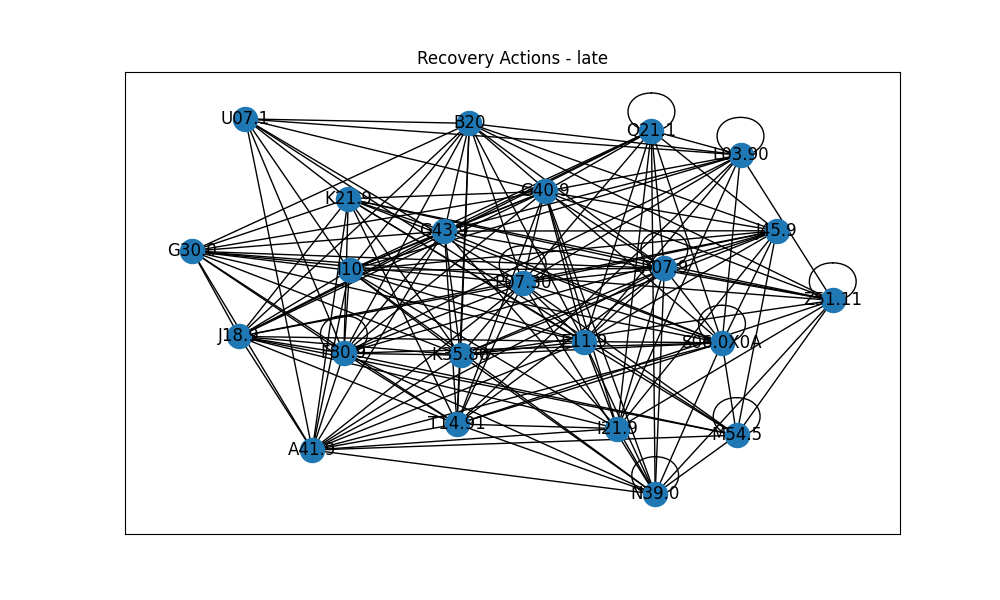
\includegraphics[width=0.32\textwidth]{recovery_late.png}
        \caption{Phase-wise recovery-promoting action patterns: early, middle, and late stages}
    \end{figure}

    \item \textbf{Confusion Matrix:} Used to visualize the classification accuracy.
    \begin{figure}[H]
        \centering
        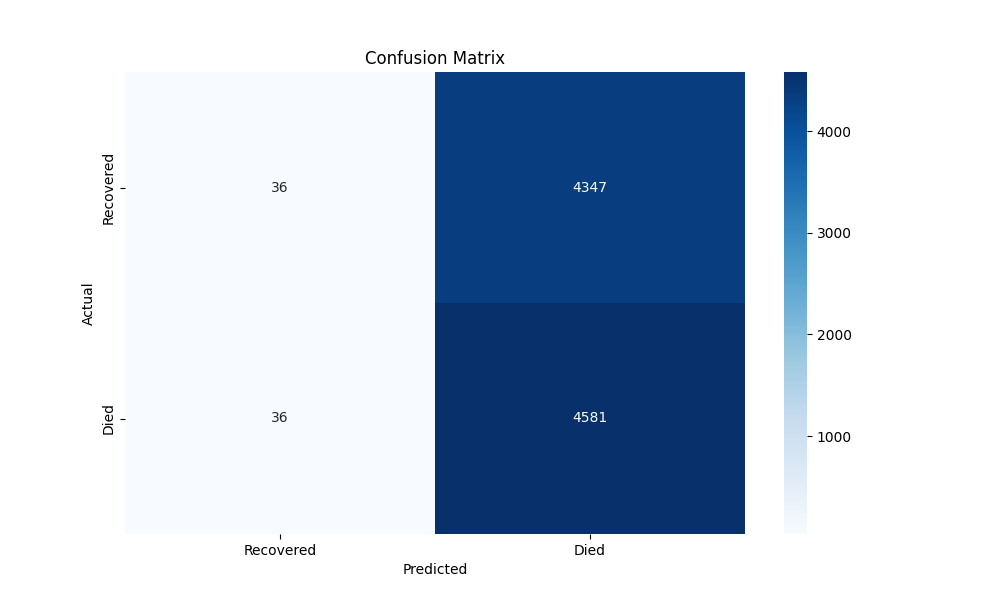
\includegraphics[width=0.5\textwidth]{confusion_matrix.png}
        \caption{Confusion matrix for classification performance}
    \end{figure}
\end{itemize}

\section{Runtime \& Complexity}
\subsection{Theoretical Analysis}
The Frequent Subgraph Mining (FSM) process consists of three key components:

\begin{itemize}[noitemsep]
    \item \textbf{Frequent Edge Detection (Algorithm 1)} \\
    \textbf{Goal:} Count all edges across graphs and retain those above frequency threshold $\tau$.
    \begin{itemize}[noitemsep]
        \item \textbf{Time Complexity:} $\mathcal{O}(E)$, where $E$ is the total number of edges across all graphs.
        \item \textbf{Space Complexity:} $\mathcal{O}(U)$, where $U$ is the number of unique edges.\\
    \end{itemize}
    
    \item \textbf{Subgraph Extension (Algorithm 2)} \\
    \textbf{Goal:} Extend frequent subgraphs using DFS-code while avoiding redundancy.
    \begin{itemize}[noitemsep]
        \item \textbf{Time Complexity:} $\mathcal{O}(k \cdot d^l)$, where $k$ is the number of frequent subgraphs, $d$ is the average degree, and $l$ is the max subgraph size.
        \item \textbf{Space Complexity:} $\mathcal{O}(C)$, where $C$ is the number of candidate subgraphs.\\
    \end{itemize}

    \item \textbf{Exact Frequency Counting (Algorithm 3)} \\
    \textbf{Goal:} Count each subgraph’s frequency using subgraph isomorphism.
    \begin{itemize}[noitemsep]
        \item \textbf{Time Complexity:} $\mathcal{O}(s \cdot n \cdot \text{ISO})$, where $s$ is the number of subgraphs, $n$ is the number of graphs, and $\text{ISO}$ is the cost of subgraph isomorphism (NP-complete).
        \item \textbf{Space Complexity:} $\mathcal{O}(s + n)$
    \end{itemize}
\end{itemize}

\textbf{Overall FSM Complexity:}

\[
\mathcal{O}(E + k \cdot d^l + s \cdot n \cdot \text{ISO})
\]

\noindent where:
\begin{itemize}[noitemsep]
    \item $E$ = total edges in dataset
    \item $k$ = number of frequent subgraphs
    \item $d^l$ = exponential growth due to subgraph extensions
    \item $\text{ISO}$ = cost of subgraph isomorphism
\end{itemize}
\vspace{1cm}
The Discriminative Subgraph Mining (DSM) process involves three main algorithms:
  
\begin{itemize}[noitemsep]
    \item \textbf{FindDiscriminativeGraph (Algorithm 4)}
\textbf{Goal:} Identify discriminative subgraphs by calling CreateDiscriminativeGraph and RelaxedCreateDiscriminativeGraph, optionally swapping positive ($R^+$) and negative ($R^-$) graph sets.

\begin{itemize}[noitemsep]
    \item \textbf{Time Complexity:} Dominated by the subroutines it invokes.
    \item \textbf{Space Complexity:} Depends on subgraph storage and intermediate results.
    \item \textbf{Initial Step:} Filters non-discriminative edges by comparing edge sets of $R^+$ and $R^-$ ($\mathcal{O}(E)$, where $E$ is total edge count).\\
\end{itemize}

    \item \textbf{CreateDiscriminativeGraph (Algorithm 5)} \\
    \textbf{Goal:} Identify discriminative subgraphs that distinguish between positive (recovered) and negative (deceased) patient outcomes.
    \begin{itemize}[noitemsep]
        \item \textbf{Time Complexity:} 
        \[
        \mathcal{O}(q \cdot n \cdot \text{ISO})
        \]
        where $q$ = number of candidate subgraphs, $n$ = number of graphs in $S_2$, and $\text{ISO}$ = cost of subgraph isomorphism (NP-complete).
        \item \textbf{Space Complexity:} $\mathcal{O}(q)$ for queue-based storage of candidate subgraphs.
        \item \textbf{Note:} The search space can grow exponentially due to recursive augmentation. \\ 
    \end{itemize}
    
    \item \textbf{RelaxedCreateDiscriminativeGraph (Algorithm 6)} \\
    \textbf{Goal:} Similar to Algorithm 5, but a subgraph is accepted if it is absent in at least $\gamma$ fraction of graphs in $S_2$.
    \begin{itemize}[noitemsep]
        \item \textbf{Time Complexity:} Similar to Algorithm 5: $\mathcal{O}(q \cdot n \cdot \text{ISO})$
        \item \textbf{Space Complexity:} Also $\mathcal{O}(q)$
    \end{itemize}
\end{itemize}

\textbf{Overall DSM Complexity:}

\[
\mathcal{O}(q \cdot n \cdot \text{ISO}) \quad \text{where } \text{ISO} \in \text{NP-complete}
\]

\noindent The overall complexity depends on:
\begin{itemize}[noitemsep]
    \item Number of candidate subgraphs ($q$)
    \item Size of graph sets ($n$)
    \item Subgraph isomorphism operations
\end{itemize}
\subsection{Emperical Analysis and Discussion }

Experiments reveal that runtime and memory usage increase rapidly with dataset size and lower support thresholds ($\tau$). The subgraph isomorphism step is the main bottleneck, especially during frequency counting. While GraMi performs well on small to medium datasets, it struggles to scale for large, dense graphs. In contrast, the relaxed DSM variant offers better control over runtime via the $\gamma$ parameter, but still inherits the high cost of isomorphism checks. Parallelization and early pruning strategies remain crucial for improving scalability.


\section{Comparative Evaluation}
\subsection*{Baseline or Prior Work}

Traditional healthcare analytics methods include collaborative filtering, decision trees, random forests, Markov models, and neural networks. Collaborative filtering approaches (e.g., CARE) face data sparsity, scalability, and cold-start issues. Decision trees and random forests require numerous trees for reliability, increasing inference latency. Markov models are limited in capturing complex dependencies in treatment sequences. Neural networks, although powerful, lack interpretability and demand large, well-labeled datasets. Clustering-based methods require heavy preprocessing and are sensitive to outliers. These limitations make such methods less suitable for handling the heterogeneous and temporally complex nature of MIMIC-type electronic health records.

In contrast, graph-based methods—specifically Frequent Subgraph Mining (FSM) and Discriminative Subgraph Mining (DSM)—model treatment data as graphs, capturing both relational and sequential patterns. They offer greater interpretability, require minimal parameter tuning, and function effectively without extensive labeled data.

\subsection*{Comparison Metrics}

Graph mining approaches outperform traditional baselines by directly modeling action sequences and identifying meaningful structures. FSM focuses on frequent patterns but often includes non-discriminative subgraphs. DSM improves upon this by extracting subgraphs strongly correlated with outcomes, enhancing signal clarity.

\textbf{Error Rates (10-fold cross-validation based on MIMIC data)}
\begin{itemize}[noitemsep]
  \item \textbf{FSM}: Phase 1 – 51.50\%, Phase 2 – 39.42\%, Phase 3 – 13.72\%
  \item \textbf{DSM}: Phase 1 – 13.37\%, Phase 2 – 8.79\%, Phase 3 – 1.53\%
\end{itemize}

These results demonstrate DSM’s superiority in predictive accuracy, interpretability, and clinical relevance compared to both FSM and conventional machine learning approaches.

\section{Enhancements}

\begin{itemize}
    \item \textbf{Experimentation with Real-World Datasets:} Attempted to obtain the actual MIMIC-IV dataset; we were not granted authority to it
    \item \textbf{Alternative Parameters or Settings:} Exchanged the alpha and beta parameters in DSM to obtain the "avoid" actions and improved recommendations
    \item \textbf{Algorithm Modifications:} Adjusted the algorithm that extracted the action types and categorised them into avoid/recommended actions, in order to fix our mortality bias. Slight improvements were found. Recommended actions were improved and more accurate.
    \item \textbf{Motivation for Enhancements:} The mortality bias doesnt allow for the best "avoid" actions, hence we wanted to make necessary changes. However we have a very solid recommendation system now.
\end{itemize}

\section{Reflection}
\subsection{Challenges Encountered}

The journey through this project involved navigating multiple challenges, which made the process both difficult and rewarding. One of the most significant hurdles was the complexity of the algorithms used, the Frequent Subgraph Mining (FSM) and Discriminative Subgraph Mining (DSM). These algorithms required a deep understanding of both their individual components and how they comapred with one another. Despite the initial complexity, we were able to break down these concepts and successfully apply them by collaborating as a team.

Another major challenge was understanding and working with healthcare data. Medical datasets are complex. The need to correctly map ICD codes and contextualize **medical conditions proved challenging. However, through continuous team discussions, we overcame these obstacles and were able to extract meaningful insights from the data.

We also faced challenges with algorithmic tuning. Setting the right thresholds to identify frequent and discriminative patterns while ensuring the algorithm remained efficient required numerous iterations. 

\subsection{Learning Outcomes}

This project provided valuable learning experiences in several areas:

\begin{itemize}
    \item Graph Mining Techniques: We gained a deeper understanding of advanced techniques like FSM and DSM, and learned how to apply these methods effectively to extract patterns from complex data.
    \item Collaboration: This project highlighted the importance of teamwork. By discussing the challenges together and brainstorming solutions, we were able to tackle difficult problems and learn from each other.
    \item Interdisciplinary Approach: Since this project is an intersection between CS and the healthcare system, it gave us a better insight into both worlds, further building on our existing knowledge on them.
\end{itemize}

\subsection{Limitations}

Despite the success of the project, there were limitations that affected the accuracy and depth of the insights:

\begin{itemize}
    \item Binary Mortality Outcome: We used a simplified binary mortality outcome, ignoring the severity of medical conditions. This limited the scope of our analysis and could have affected the recommendations provided by the model.
    \item ICD Code Limitations: The ICD codes used in this project might not capture the full clinical context (e.g., lab values), which could potentially impact the model's ability to make highly accurate predictions.
    \item Static Thresholding: The static thresholds used for identifying frequent patterns might have missed more dynamic and subtle patterns that evolve over time.
    \item Access to MIMIC Dataset: Due to the rigorous application process, we were not able to get access to the actual dataset used in this research. However, we were able to build a sample dataset with all the necessary columns and data
\end{itemize}

\subsection{Future Work}

This project has laid the groundwork for several exciting possibilities in healthcare data models. In the future, we could:

\begin{itemize}
    \item Integrate Temporal Features: Adding temporal features could allow the model to understand how patient conditions evolve over time, enabling more accurate predictions and recommendations.
    \item Leverage Attention-Based Graph Neural Networks (GNNs): GNNs could provide a richer representation of patient data, making the model more capable of handling complex and diverse healthcare datasets.
    \item Incorporate Reinforcement Learning: Future work could explore reinforcement learning to recommend specific treatment actions, enabling a more dynamic, personalized approach to patient care.
    \item Expand Dataset Diversity: Incorporating data from multiple hospitals or regions would improve the generalizability of the model and ensure that it works effectively in various healthcare settings.
\end{itemize}

\subsection{Conclusion}

Overall, this project has been a rewarding exploration of how advanced graph mining techniques can be applied to healthcare data to extract meaningful patterns that can assist in decision-making. Despite the challenges, the insights we derived showed the potential of such methods in transforming healthcare practices. The next step is to expand the scope of this work to address the limitations and explore further innovations that could revolutionize healthcare systems, ultimately improving patient outcomes globally.


\section{Github Repositary Update}
To align with Checkpoint 4 requirements, the following updates have been made to our project repository:

\begin{itemize}[noitemsep]
    \item \textbf{Checkpoint 4 Folder:} Added LaTeX source files, compiled PDF of the report, presentation link and pdf. 
    \item \textbf{README.md:} Updated to reflect current progress, report summary, and key insights as well as a guide to run the code
    \item \textbf{Other Folders:} Folders of previous checkpoints, research materials, src, and data are updated. 
    
\end{itemize}
The repository remains clean, well-structured, and adheres to version control best practices.

\end{document}
